\setcounter{chapter}{0}
\chapter{Physics of gamma-ray bursts.}
\section{Introduction}
\textbf{what are gamma-ray bursts?}\\
Gamma Ray Bursts (GRBs) are Sudden ,intense , bright and non-repeative flashes of gamma-ray
photons of energy in the gamma -ray band (keV - GeV) lasting from a few tens of milliseconds  to several minutes.They are the fastest extended objects of Nature, that injecting large amount of energy of order $10^{55}$ergs or $ 10^{47} $ joules from very small compact region in a few seconds at cosmological distance.The energy released for a few second to hundred seconds comparable to the energy that  the Sun will emit in its entire 10 billion years of life time. Furthermore,the overall observed fluence ranges from $10^{-4} $ ergs/$ cm^{2}$ to $ 10^{-7} $ ergs/ $ cm^{2} $ (shown in fig 1.2 , section 1.2 ), that corresponds to the isotropic equivalent luminosity of $ 10^{48} $  to  $10^{54} $ erg $ s^{-1} $ \citep{1}.\\\\
Gamma Ray Bursts (GRBs) are at the intersection of many different areas of astrophysics: they are relativistic events connected with the end stages of massive stars; they reveal properties of their surrounding medium and of their host galaxies; they emit radiation from gamma-rays to radio wavelengths, as well as possibly non-electromagnetic signals, such as neutrinos, cosmic rays and gravitational waves. Due to their enormous luminosities, they can be detected even if they occur at vast distances, and are therefore also of great interest for cosmology \citep{2}.\\\\
 During  explosions, ultra relativistic jets are produced accompanied by an intense gamma-ray flashes called prompt emissions that outshine all the sky at very high red shifts.These prompt emissions are often followed by afterglow signals across the electromagnetic spectrum from X-ray to radio wavelengths covering timescales from tenth of seconds up to several months or more \citep{1,2}.\\\\
GRB  events are  classified   as being  either  long  (lasting > 2) or short (lasting < 2 s), separated  by  the length  of durations $T_{90} \sim 2 $sec, and  spectral hardness of their prompt emissions, with long  GRBs (LGRBs) believed to be associated with the  deaths of collapsed  massive  stars, whilst  short  GRBs (SGRBs) more likely to be  the  result of  either  the  merger of  binary  neutron  stars (BNS) or the  merger  of  a neutron  star  with  a black  hole (NS-BH) \citep{3}.\\\\
Due to their huge radiated energies, GRBs can be observed up to $z  \sim 10$, there 
fore they are very powerful cosmological tools, complementary to other probes
such as SN-Ia , clusters etc.The correlation between spectral peak photon
energy Ep,i and intensity (Eiso, Liso, Lp,iso) is one of the most robust and intriguing properties of GRBs and a promising tool for measuring cosmological parameters \citep{2, 3}.
\section{Historical Discovery of gamma-Ray bursts }
Gamma-ray bursts (GRBs) were first discovered unexpectedly during the Cold War
in the late of $1960_{s}$  by the Vela military satellites that  were equipped with detectors of gamma-rays, X-rays and neutrons and launched by USA Air Force in collaboration with the Los Alamos National Laboratory.The first event was recorded in 1967.After verification, it was clear that gamma radiation was not of human origin, nor even terrestrial. However,the existence of Gamma-ray flashes coming from cosmos was  announced the first event after six years in 1973 dating back to july 2,1967       \citep{4}.\\\\ 
The stuy of GRBs physics mainly led by observations with help of improved detecting instruments on satellites to monitor phenomena in the universe in relation to  Gamma- ray emissions.  Prompted by the instrumental progress from time to time, the story of obsrevational research of GRBs from early time to recent  classified in five eras  \citep{4} \citep { 5}.\\\\
\subsection{Dark era (1967-1990)}
 The first gamma -ray burst discovered  named as " GRB 670702" that  detected by vela satellite (see fig 1.1).In the name " GRB 670702", the first two digits represent the burst year, the middle two  and the last two digits represent month and the last two digits date of the burst. If more than two events of bursts were happened in one day, they labeled to identify them  using  English letters alphabetically. \citep {4} \citep { 5}.\\\\
\begin{figure}[h]
\begin{center}
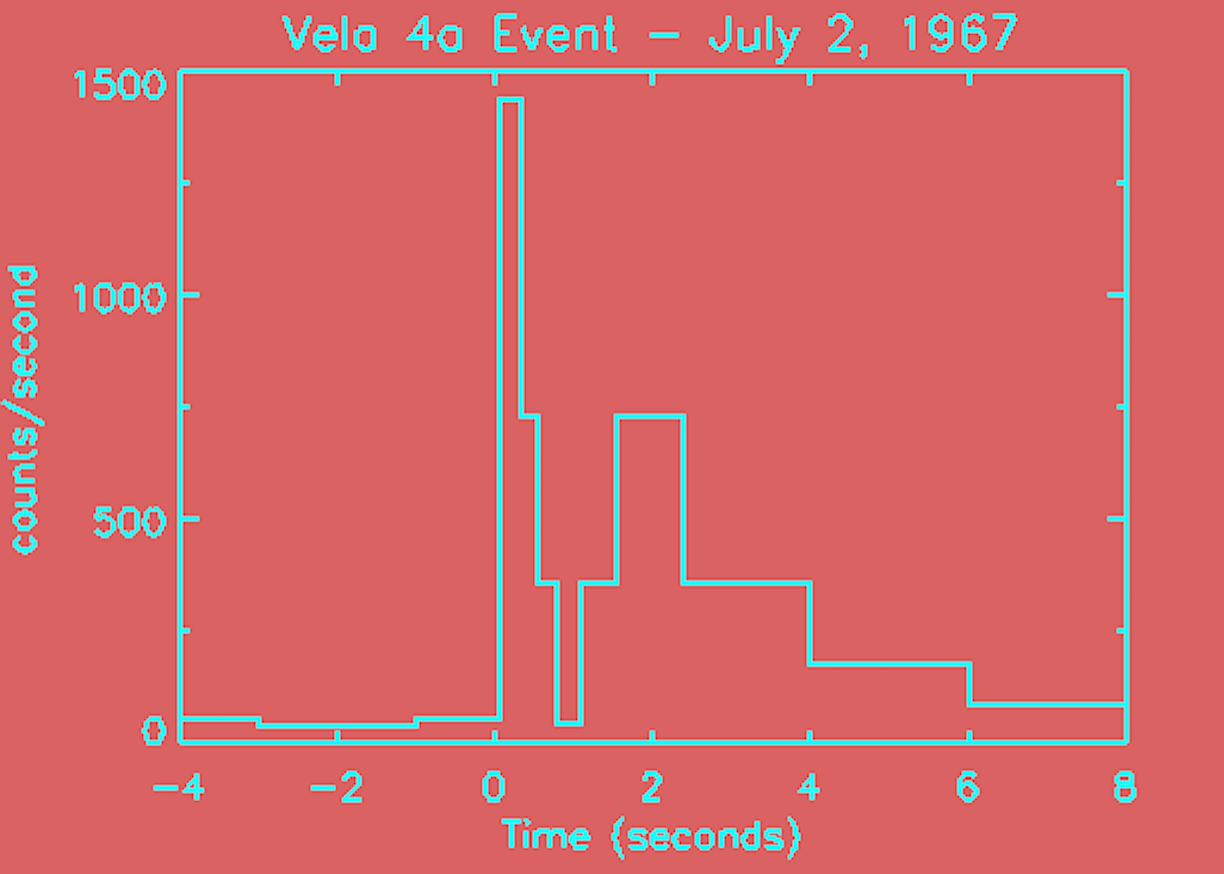
\includegraphics[scale=0.2]{Figures/fig1.png}
\caption{Light curve of the first GRB ever detected by Vela. Two separate pulses can be identified over a duration of less than 10 seconds \citep{4}}
\end{center}
\end{figure}
After the first discovery , the series of vela satellites were launched ,and more than 70 GRBs were detected. These earliest observational result of GRBs only consists several structures “spikes” were found in Gamma-ray band ,but no way to identify their location. However,after series of  vela satellites were launched with improved detecting instruments ,the origions of GRBs belived to be out side the solar system by offset information \citep{4} \citep { 5}.\\\\
The fundamental questions of the era were : Where are GRBs come from ?   What is the source of such flashes of light? By what mechanisms ? do they appear in our galaxy, the Milky Way, or in more distant galaxies ? To answer such questions More than one hundred models were proposed to explain the origin and  production mechanisms of GRBs. However, only a few of them were explaining  that GRBs events occur at cosmological (at far distances). On the other hand, the majority of the models were indicating that the events of GRBs closer to the Earth (galactic origin) apparently to overcome the energy out put. During the era, the detection and interpretation of GRBs were not progressive due to lack of improved detecting instruments ,however  GRBs as new field of science was opened at the end of the era\citep{4}\citep{6}. \\\\
\subsection{BATSE era (1991-2000)}
The Burst And Transient Source Experiment (BATSE) was the early advanced space detecting instruments that carried on the Compton Gamma-Ray Observatory (CGRO), that capable to map Gamma-ray sources from almost the entire sky in energy range of (20keV - 2MeV ).The contributions of BATSE in its nine years successful operations were:\\
$\bullet$ At its early operation in 1991,the apparent isotropic spatial distributions of 2704 GRBs were confirmed (see fig 1.2 ) ,and then the cosmological origin of GRBs was accepted by astronomers although the debate between galactic and cosmological origin continued until BeppoSAX. \citep{5}\citep{7}.\\\\
The fig shows,the  distribution is « isotropic »: the bursts are distributed randomly on the map indicating that they are either very close to the Earth, or very far, of extragalactic origin. No concentration of bursts along the plane of the Milky Way, symbolized on the map by the horizontal center line, appears. This most likely excludes candidates from our galaxy.\\\\
\begin{figure}[h]
\begin{center}
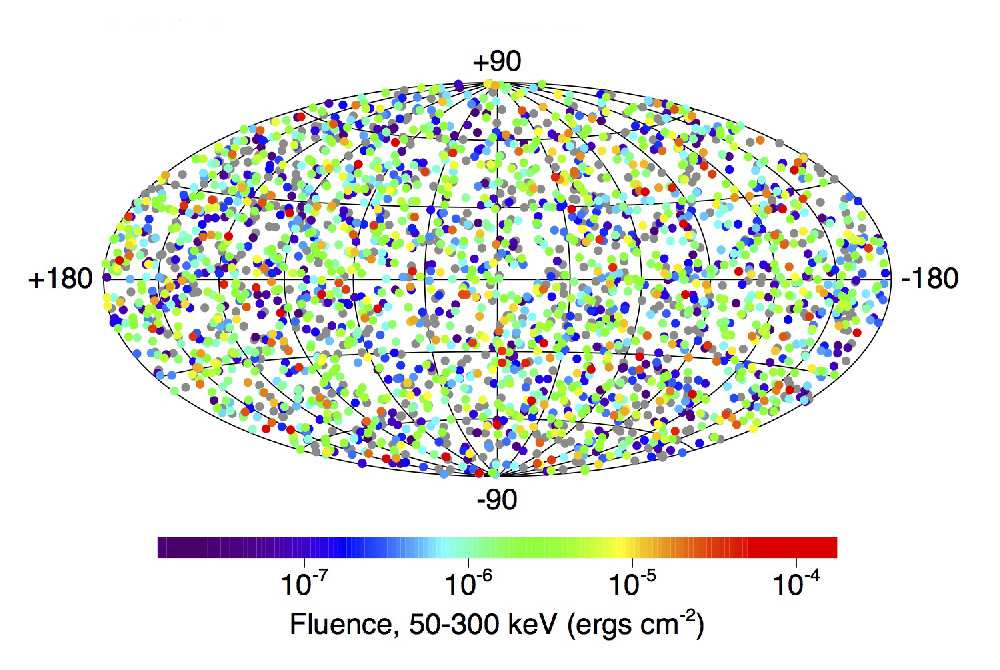
\includegraphics[scale=0.4]{Figures/fig2.png}
\caption{The distribution of all 2704 GRBs detected by BATSE satellite: they are clearly isotropically distributed \citep{7}. }
\end{center}
\end{figure}
$\bullet$Fireball model as the theoritical tool to explain the huge amount of energy   drived from observed flux and fast time variability.\\
$\bullet$ confirm  the classification GRBs into two types (short and long GRBs) according to  bimodal distribution of durations parameter $ T_{90} $.\\
$\bullet$provide database of GRBs, their spectral and temporal properties \citep{5}\citep{7}.\\\\
\textbf{limitations of BATSE}\\
$\bullet$unable to cassify  diversities(single spikey pulses,smooth with or multiple peaks,very erratic,chaotic and spikey).\\ 
$\bullet$ BATSE’s observations remain limited to gamma-rays alone,no follow-up observations at other longer wavelengths \citep{5}\citep{6} \citep{7}.
\subsection{Bepposax era (1997-2000)}
Bepposax equipped with improved instruments on satellite launched in 1997. It was designed to detect long -living afterglows from X-ray to  radio wavelength.The contributions of BATSE in its seven years operations were:\\
$\bullet$ confirm the precise location of the burst in the X-rays rapidly transmitted  and also discoverd weak and decreasing signals.This was the late-time, weaker emission radiates in the X-rays, optical and radio waves. \\
$\bullet$ Opened a new era for the current understanding of the mystry of GRBs.\\
$\bullet$ predicted the existence of GRBs afterglow in longer energy bands (from optical to radio wave length).\\
$\bullet$Provide clues for GRB-SN possible connection , which was latter confirmed by
HETE-2 and Swift that support collapser model and explosions of massive star
of wolf-Rayet (WR),leaving behind BH.\\
$\bullet$Provide crucial informations on the progenitors of GRBs.\\
$\bullet$X-ray flash as new class of GRB with less-lumineous and low redshift identified from traditional GRBs \citep{4} \citep{7}.\\\\
\textbf{limitation of Beppo-sax}\\
$\bullet$unable to show the canonical behavior of x-ray afterglow which was later shown by swift \citep{5}.\\\\
\subsection{Swift era(2004-now)}
The Swift was a robotic spacecraft. It was launched into orbit on November 20, 2004 
and  orbits at 567 km x 585 km with a period of 95.9 min.is to investigate four phenomena : GRB progenitors, different physical processes underlying different GRB class observations, the interaction between the blastwave and its surroundings, and the early Universe through GRBs. Swift also aimed to investigates other non-GRB-related phenomena. It was the first multi wavelength mission for the study of GRBs, being elaborated by an international collaboration.In its ten years operations , Swift detected more than 2300 GRBs \citep{4} \citep{6}.\\\\
Swift designed to detect and study the two phases of GRBs : prompt and afterglow emissions , and equipped with  three sophisticated detecting instruments working together to observe GRBs and their afterglows in the gamma-ray, X-ray, ultraviolet and Optical wavebands.(see fig 1.3) The  instruments and their functions described below:\citep{8}\cite{9}.\\
\begin{figure}[h]
\begin{center}
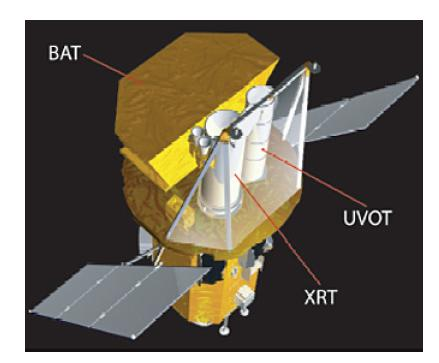
\includegraphics[scale=0.4]{Figures/fig3.png}
\caption{Schematic view of the swift satellite(Gehrels et.al 2004).The size of Mask of BAT is $2.7m^{2}$  \citep{7}} 
\end{center}
\end{figure}
\textbf{Burst Alert Telescope (BAT)}.\\
BAT detects GRB event and computes its coordinate (position) in the sky and
locates the position of each event with an accuracy of 1 - 4 arcminutes with in 15
seconds. This position immediately relayed to the ground and rapid slew-ground
based telescope catches the informations.\\\\
\textbf{X-Ray Telscope (XRT)}\\
It takes image and perform spectral analysis of the GRB afterglow. This provides
more precise postion of GRB with a typical error circle of approximation 2 arcseconds
radius. The XRT also used to perform long term monitoring of GRB afterglow light
curves and operated in energy range of 0.2 keV - 10 keV .\\\\
\textbf{ Ultra Violet optical Telescope (UVOT)}\\
UVOT used to detect optical afterglow and provide a sub-arcseconds position. It
also used to provide longer wave length follow ups of GRB afterglow light curves.
 Swift has been a great success in its observations. results include:\\
$\bullet$ Revealed unusual yet “canonical" X-ray afterglow behavior of X-ray flaring activity during the afterglow phase.\\
$\bullet$ show the transition from prompt to afterglow emission.\\
Finally, it detected the high-z GRBs such as 050904,080913 and 090423,which
were the most distant cosmic explosions \citep {5} \citep{7}.\\\\
\subsection{Fermi era (2008-now)}
 Fermi designed to focus on prompt emissions phase of GRBs by using  much higher energy ranges (8keV - 300keV) than swift (15keV -150keV).It carries on board two types of detectors known to be  Gamma-Ray Burst Monitor (GRBM ) and Large Area Telescope (LAT).They provide unprecedented spectral coverage for seven orders of magnitudes of energy from 8 keV to 300 GeV.Fermi made Significant progresses for the current understanding of origin of GRBs.\\ 	The contributions of Fermi since launched were:\\
$\bullet$ The existence of three elemental spectral components (Band function-like, thermal and extra non-thermal power-law components ) in GRB spectra was confirmed.\\
$\bullet$ Suggest that the featureless Band function spectra extended from keV to Gev
band a Poynting-flux-dominated flow.\\
$\bullet$ Explain the existence of thermal components in some GRBs(e.g GRB 5090902B)
due to hot fireball without strong magnetization.\\
$\bullet$ The delayed onset of GeV emission in some LAT GRBs suggests that there likely be a change of either particle acceleration condition or the opacity of the fireball during the early prompt emission epoch.\\
$\bullet$ confims that long lived GeV emission is likely of external origin, while GeV emission during the prompt phase, on the other hand is likely of internal origin \citep{10} \citep{11}.
\section{Classification of gamma-ray bursts}
Based on the bimodal distributions of durations $ T_{90}$ or $ T_{50}$ of prompt phase or hardness ratio , GRBs have been catagorized in to two groups: short/hard and long/soft GRBs. The duration of GRB,$ T_{90} $ or $ T_{50}$  , is defined by the time interval over which 90 \%  or  50 \%  of the burst fluence is detected respectively. The typical duration of a GRBs is $\sim $ 20 - 30  seconds for long bursts and $\sim $ 0.2 - 1.3 seconds for short bursts. Observationally the durations of GRBs can be in a range of 5 orders of magnitude, i.e, from $\sim $ $ 10^{-2} $ s  to $\sim $ $ 10^{3} $ s. The bimodal distribution of $ T_{90} $ has been used to identify the two categories of GRBs, namely, “long” or "soft" ($ T_{90}$ $\geqslant $ 2  s ) and “short” or " hard "$( T_{90}$   $\leqslant$ 2 s ) (see Fig1.4 ). Instrumentally ,  $T_{90}$  or  $T_{50} $ depends on the energy band and the sensitivity limit of the detector.
\begin{figure}[h]
\begin{center}
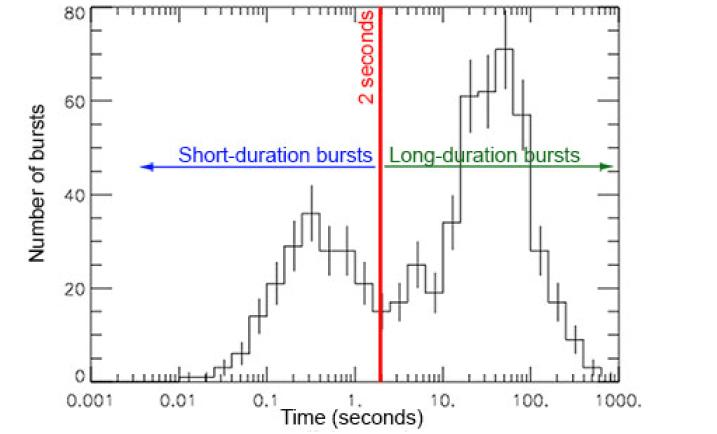
\includegraphics[scale=0.4]{Figures/fig4.png}
\caption{The GRB classification (long and short) distribution.}
\end{center}
\end{figure} 
Theoretically, there are three timescales which may be related to the observed GRB duration $ T_{90} $:\\
(1) central engine activity time scale $t_{eng}$\\
(2) relativistic jet launching time scale $t_{jet} $\\
(3) energy dissipation time scale $t_{dis}$ . Then, the observed GRBs duration $  T_{90}$ should satisfy: \citep{5}
\begin{equation}
T_{90} \leq \delta  t_{dis} \leq\delta t_{jet} \leq \delta t_{eng} 
\end{equation}
\subsection{short/hard gamma-ray bursts} 
Short/Hard gamma ray bursts (SGRBs) are events with a duration $T_{90}$ less than 2
seconds and account for about 30\% of the total gamma ray bursts.They are highly
energetic /hard gamma-rays when compared with their long burst counterparts.For
many years short-hard GRBs were not deeply researched as long GRBs.As a result,
study of short-hard GRBs (SHBs)limited. However,one year after swift launch, in
2005 a breakthrough occurred following the first detections of SHB afterglows \citep{5}\citep{6}.\\\\
The swift observations established that SHBs are cosmological relativistic sources
that, unlike long GRBs, do not originate from the collapse of massive stars, and
therefore constitute a distinct physical phenomenon. One viable model for SHB
origin is the coalescence of compact binary systems , in which case SHBs are the
electromagnetic counterparts of strong gravitational-wave sources. In this burst,
the conversion of energy into gamma- rays decreases as the burst progresses.There
is no radio, optical, or x-ray counterpart has found for any short burst \citep{5}.
\subsection{long/soft gamma-ray bursts} 
Another subclass of GRBs that account for 70\% and have a duration of greater than
2 seconds are classified as long/soft GRBs (see fig 1.4 above). All long bursts display x-ray afterglow and about one-half as radio or optical afterglows.In long duration bursts energy conversion appears to remain constant through burst.Their creation linked to a young galaxies with rapid star formation and to a core collapse of supernova as well.This is unambigeously associating long GRB with the death of massive stars.Observations of LGRB afterglow at high red shift ,are also consistent with the GRB having originated in star-forming regions \citep{6}.
\subsection{Ultra long gamma-ray bursts (ULGRBs)}
GRBs with highly a typical durations of more than 10,000sec called ultra-long
gamma-ray bursts (ulGRBs).They are the tail end of the standard long GRBs that
caused by the collapse of a blue supergiant star,tidal distruption events or a new
born magnatar. They have been proposed to form a new third class of GRBs. One
explanation which has been proposed for their ultra-long duration is that they
could have progenitors differ from classical GRBs in that: they could be produced
either by the core collapse of a low-metallicity supergiant blue star, the birth of a
magnetar following the collapse of a massive star or the collapse of a Pop III star.In any case, it is clear that the durations of these bursts make them so peculiar that they need further studies \citep{10} \citep{11}.
\section{Gilobal properties of GRBs}
Two distinct global properties of “classical GRBs” began to emerge—the intensity
/brightness and the angular / location distributions—both are important implications
for the distance scale of GRBs and hence their origin.
\subsection{Intensity distribution}
The brightness distribution of GRBs appeared to show that we were seeing out
to the edge of the GRB population:there were too few faint GRBs relative to the
number expected if GRBs were uniformly (“homogeneously”) distributed in space.
Brightness was most straight forwardly measured as the peak flux (P , with units
[erg $ s^{-1} $ $cm^{-2} $ ]) in the light curve of a GRB. The brightness distribution is usually measured as the number, N(>P ), of GRBs brighter than some peak flux P per year. If the peak luminosity (L, with units [erg $ s^{-1} $]) of all GRBs is the same, then, using the $ \frac{1}{r^{2}} $ law, for a given flux P we would see all the GRBs within a maximum distance:\citep{7} \citep{12}.
\begin{equation}
d_{max}\approx\sqrt{\frac{L}{4\pi P}}\varpropto P^{\frac{-1}{2}}
\end{equation}
All the GRBs to that distance would be brighter than P by construction. The
number of GRBs we would detect to that brightness (or brighter) in one year would
just be the volume times the intrinsic rate (R, in units of [event $yr^{-1}$ per volume element]):$ N (> P ) \propto V \times R \propto R \times d_{max} \propto R \times P^{\frac{-3}{2}}$.  So with a homogeneous distribution, we expect that the number of faint GRBs N should grow as a power law proportional to $P^{\frac{-3}{2}} $, where the constant of proportionality scales directly related to the intrinsic rate R: for every ten times fainter in flux we observe, we would nominally expect about thirty-two times more GRBs. While this was indeed seen for the brightest events,there was a flattening at the faint end of the brightness distribution. This flattening was highly suggestive that we were seeing the “edge” of the GRB distribution in space,an important clue in understanding the distance scale. But without knowing the intrinsic luminosity L, we could only infer the shape of the distribution, not the scale. It was like seeing a picture of a building but not knowing if it was of a miniature in a snow globe or the life-sized version \citep{7}\citep{12}.\\\\
\subsection{Angular distribution}
The locations of GRBs on the sky appeared to be randomly (isotropically) distributed:
that is, there was no indication that any one direction on the sky was especially
more apt to produce GRBs than any other (see fig1.2 in section 1.1).If GRBs were
due to neutron stars strewn through out the disk of the Galaxy, for instance, the
locations of GRBs on the sky should have been preferentially located near the
Galactic plane (as is seen with SGRs). If associated with older stars in the roughly
spherical “bulge” of the Milky Way, GRBs would have been preferentially located in
the direction toward the Galactic center and less so toward the opposite direction.
The inference that the Sun was roughly at the center of the GRB distribution in
space,while casting aside some models, still allowed for a variety of distance scales: from a fraction of a light year to billions of light years \citep{7}.
\section{Statement of the problems}
As mentioned in section 1.1 above ,to study the mystry and  phenomenology of Gamma-ray bursts , several  satellites ( from Vela at early time  to  fermi and others at recent time ) equipped  with different instruments (telescopes ) have been launched. Among those satellites , swift was open new era  for the current understanding and development of gamma ray researches.Swift missons  detected  the prompt and the afterglow emission phases of grb.  Moreover, the temporal and spectral behaviors as well as  properties of x-ray and optical  light curves of most grb also studied. However, as far as my search /review litrature is concerned, there is a gap knowledge that explaining more about canonical x-ray light curves:\\
$\bullet$ Does x-ray afterglow the results of internal or external shocks or both? \\
$\bullet$ What parameters / variables responsible for the variations of temporal and spectral indices  of canonical x-ray ;\\
$\bullet$ what is the implications the variations both indexs.\\
In this thesis, I emphasized on the theoritical and observational properties of canonical X-ray afterglow light curves  qualitatively and quantitatively.\\\\
Regarding this work the unclear ideas or un answered questions are listed below. Among these:\\
(1) what are the cause of canonical x-ray light curve of afterglow grb?\\
(2) what are the proginators of canonical x-ray light curves?\\
(3) Did the  value  of temporal index  of any random GRB confirmed to the proposed value in all phases canonical x-ray LCs ?\\
(4) Could some of the breaks at the end of the plateau phase actually be jet break
or late steep decay phase? The goal of this thesis is  attempt to explain and give answers for these questions.
\section{Objectives and thesis outline}
\textbf{General objective}\\
 To study how characterstics of light curves gamma ray bursts affected by some  paramerters or variables such as flux ,luminosity and  time.\\\\   
\textbf{specific objectives}\\
$\bullet$To explain the  cause and effect  for the  variations of light curves of  prompt and afterglow phases.\\
$\bullet$To compare / contrast the proposed values of temporal and spectral  indices of x-ray afterglow with/to the calculted values.\\
$\bullet$To describe the implications of  temporal ($\alpha$) and spectral ( $ \beta $) indices gamma -ray afterglows.\\
\textbf{Thesis outline}\\
 Hereafter, I point out the outline of the thesis. In chapter 1 above, the  background of gamma -ray physics  and a short historical discoveries /explorations/, grb as well as  gradual development of them for the past  five decades would be discussed. Chapter 2,mainly focused on the production  /  emission mechanisms of gamma-ray bursts,  theoritical and obsevational properties of grb explained using standared fireball moedels. Furthermore,the  dissipative process( matter- dominated phase ) and Radiative process ( radiation - dominated phase) of gamma -ray emission  mechanisms are  explained indetaild.\\\\
In chapter 3, I address  methodology / methods , and  models tools  used to analyze the temporal and spectral propeties of canonical x-ray light curves in swift/XRT for some seleted gamma-ray bursts with red shifts two or more breaks.
In chapter 4, I discuss on achieved results /findings  with proposed values by comparing / contrasting  using tables and charts.Finally,I forward  a brief summary or review of the enlightenment of this work, as well as a hint for future research in the last chapter. 
